\documentclass{article}

\usepackage{amssymb}
\usepackage{amsmath}
\usepackage{amsfonts}
\usepackage{mathtools}
\usepackage{esint}
\usepackage{hyperref}

\title{MATEK 2 Jegyzet}
\author{Krusóczki Ádám}
\date{\today}

\renewcommand{\contentsname}{Tartalom}

\begin{document}

\tableofcontents

\newpage

\maketitle


\section{Előszó}

Ez a jegyzet főképp a BME VIK villamosmérnöki szak Matematika II. tár\-gyá\-ra ké\-szült, de hasz\-nál\-hat\-ja bárki, 
akinek jegyzetre van szüksége, lineáris algebából, végtelen sorokból vagy többváltozós függvényekből. Ebben a jegyzetben nincsen részletesen
leírva a lineáris algebra sok része (egyenletrendszerek, Gauss-Jordan elimináció, determinánsok, mátrixok, mátrixműveletek), mert ezeket a témákat a Számítástudomány
alapjai tárgyban tartották nekünk, amihez volt kidolgozott jegyzetünk. 

\vspace{4mm}

A hatványsorokig ellenörzött, a matematika gyakorlatvezetőnk által, de e\-lő\-for\-dul\-hat\-nak hibák a jegyzetben! A hibák jelzését nagyon megköszönöm,
erre a jegyzet \href{https://github.com/krusoadi/tex_notes}{GitHub repository}-jában van lehetőség (Issues menüpont alatt). 

\vspace{4mm}

Jó tanulást (és sok szerencsét a vizsga/zh-hoz)!

\newpage

\section{Lineáris algebra}

\subsection{Ismétlés}

\subsubsection{Egyenes egyenlete síkban}
    Adott $P(x_0, y_0)$ és $\underline{n} = \left( A, B \right)^T$ \textbf{normálvektor}. Ekkor az egyenes egyenlete:

\begin{equation*}
    A(x-x_0) + B(y-y_0) = 0
\end{equation*}

\subsubsection{Egyenes egyenlete térben}
    Adott $P(x_0, y_0, z_0)$ és $\underline{v} = \left( A, B, C \right)^T$ \textbf{irányvektor}. Ekkor az egyenes egyenlete:

\begin{equation*}
    \frac{x-x_0}{A} = \frac{y-y_0}{B} = \frac{z-z_0}{C}
\end{equation*}

\subsubsection{Sík egyenlete}
    Adott $P(x_0, y_0, z_0)$ és $\underline{n} = \left( A, B, C \right)^T$ \textbf{normálvektor}. Ekkor a sík egyenlete:

\begin{equation*}
    A(x-x_0) + B(y-y_0) + C(z-z_0) = 0
\end{equation*}

\subsubsection{Sklaláris/Diadikus/Vektoriális szorzat}
Adott 
\begin{align*}
    \underline{a} &= \begin{bmatrix} x_0 \\ y_0 \\ z_0 \end{bmatrix} &
    \underline{b} &= \begin{bmatrix} x_1 \\ y_1 \\ z_0 \end{bmatrix}
\end{align*}
vektorok. Ekkor a \textbf{skaláris szorzatuk}:
\begin{equation*}
    \left\langle \underline{a}, \underline{b} \right\rangle = \underline{a} \cdot \underline{b} = \underline{a}^T\underline{b} = x_0x_1 + y_0y_1 + z_0z_1
\end{equation*}

\newpage

És a \textbf{diadikus szorzatuk}:

\begin{equation*}
    \underline{a} \circ \underline{b} = \underline{a}\underline{b}^T = \begin{bmatrix} x_0 \\ y_0 \\ z_0 \end{bmatrix} \begin{bmatrix} x_1 & y_1 & z_1 \end{bmatrix} = \begin{bmatrix} x_0x_1 & x_0y_1 & x_0z_1 \\ y_0x_1 & y_0y_1 & y_0z_1 \\ z_0x_1 & z_0y_1 & z_0z_1 \end{bmatrix}
\end{equation*}

Végül a \textbf{vektoriális szorzatuk}:
\begin{equation*}
    \underline{a} \times \underline{b} = det\begin{bmatrix} e_1 & e_2 & e_3 \\ x_0 & y_0 & z_0 \\ x_1 & y_1 & z_1 \end{bmatrix}
\end{equation*}

Ahol $e_1, e_2, e_3$ az egységvektorok. A vektoriális szorzat iránya merőleges mindkét vektorra.

\subsection{Vektorterek}

\subsubsection{Definíció}

Azt mondjuk, hogy $V$ vektortér $\mathbb{F}$ számtest felett, ha értelmezett a következő két művelet:
\begin{enumerate}
\item $+:V\times V\rightarrow V \qquad +\left(\underline{u},\underline{v}\right)\vcentcolon = \underline{u}+\underline{v}\in V$:
\begin{itemize}
\item $\forall \underline{u},\underline{v}\in V \qquad \underline{u}+\underline{v}=\underline{v}+\underline{u}$
\item $\forall \underline{u},\underline{v},\underline{w}\in V \qquad \underline{u}+\left(\underline{v}+\underline{w}\right)=\left(\underline{u}+\underline{v}\right)+\underline{w}$
\item $\exists!0\in V \qquad \forall \underline{u}\in V \qquad \underline{u}+0=\underline{u}$.
\item $\forall \underline{u}\in V \exists!-\underline{u}\in V \qquad  \underline{u}+\left(-\underline{u}\right)=0$.
\end{itemize}
\item $\cdot:\mathbb{F}\times V\rightarrow V \qquad \cdot\left(\lambda,\underline{u}\right)\vcentcolon = \lambda\underline{u}\in V$:
\begin{itemize}
\item $\forall \lambda,\mu\in\mathbb{F}\qquad \forall \underline{u}\in V \qquad \lambda\left(\mu\underline{u}\right)=\left(\lambda\mu\right)\underline{u}$
\item $\forall \lambda,\mu\in\mathbb{F}, \forall \underline{u}\in V \qquad \left(\lambda+\mu\right)\underline{u}=\lambda\underline{u}+\mu\underline{u}$
\item $\forall \lambda\in\mathbb{F}\qquad\forall \underline{u},\underline{v}\in V \qquad \lambda\left(\underline{u}+\underline{v}\right)=\lambda\underline{u}+\lambda\underline{v}$
\item $\exists!1\in V \qquad \forall \underline{u}\in V \qquad 1\underline{u}=\underline{u}$.
\end{itemize}
\end{enumerate}

\subsection{Lineáris függetlenség, Generátorrendszerek, Bázisok}

\subsubsection{Lineáris függetlenség}
Legyenek $\underline{v}_1, \underline{v}_2, \ldots, \underline{v}_n$ vektorok. Ezek akkor alkotnak lineárisan független rendszert, ha:

\begin{equation*}
    \sum_{i = 1}^{n}\lambda_i\underline{v}_i = \lambda_1\underline{v}_1 + \lambda_2\underline{v}_2 + \ldots + \lambda_n\underline{v}_n = \underline{0} \Leftrightarrow  \lambda_1 = \lambda_2 = \ldots = \lambda_n = 0
\end{equation*}

\subsubsection{Generátorrendszerek}

Legyenek $\underline{v}_1, \underline{v}_2, \ldots, \underline{v}_n$ vektorok. Ezek akkor alkotnak generátorrendszert \textbf{V vektortérben}, ha:

\begin{equation*}
    \forall \underline{w} \in V: \underline{w} = \sum_{i = 1}^{n}\lambda_i\underline{v}_i
\end{equation*}

\subsubsection{Bázisok}

Legyenek $\underline{v}_1, \underline{v}_2, \ldots, \underline{v}_n$ vektorok. Ezek akkor alkotnak bázist $\mathbf{V}$ vektortérben, ha:

\begin{enumerate}
    \item Generátorrendszert alkotnak
    \item Lineárisan függetlenek   
\end{enumerate}

Bármely vektor kifejezhető egyértelműen a bázis vek\-tor\-ok li\-ne\-ár\-is kom\-bi\-ná\-ci\-ójaként.

\subsubsection{Dimenzió}

Egy vektortér dimenziója a bázisának számossága. Jelölése: $\mathbf{dim(V)}$.

\subsubsection{Rang}

Egy vektortér rangjának száma a benne lévő független vektorok maximális száma. Jelölése: $\mathbf{rank(V)}$.

\subsubsection{Altér} 

A V vektortérnek W altere, ha $W \subset V$ és W is egy vektortér a V-beli mű\-ve\-le\-te\-kre. Jelölése: $W \leq V$.

\newpage

\subsubsection{Ortogonális bázis/Gram-Schmidt ortogonalizáció}

Az ortogonális bázis egy olyan bázis ahol a bázisvektorok páronként me\-rő\-le\-ges\-ek egy\-más\-ra. A Gram-Schmidt ortogonalizáció egy olyan eljárás, amely egy tetszőleges bázist ortogonális bázissá alakít.

Adott $\underline{u}$ és $\underline{x}$ vektorok. Ekkor az $\underline{x}$ vektor $\underline{u}$ vektorra vetítése a kö\-vet\-ke\-ző\-kép\-pen számítható:

\[
\mathrm{proj}_{\underline{u}}\,\underline{x} =\frac{\langle \underline{u} ,\underline{x} \rangle}{\|\underline{u}\|^2} \underline{u}
\]

ahol $\langle \underline{u} ,\underline{x} \rangle$ a két vektor skaláris szorzatát jelöli. 
\vspace{4mm}
\newline Az eljárás lényege, hogy az első vektor marad, a második vektort kivonjuk az első vektorra vetített második vektorból, a harmadik vektort pedig kivonjuk az első két vektorra vetített harmadik vektorból, és így tovább.

\begin{align*}
    \underline{v}_1 &= \underline{u}_1 & e_1 = \frac{v_1}{\left\lVert v_1\right\rVert}\\
    \underline{v}_2 &= \underline{u}_2 - \mathrm{proj}_{\underline{v}_1}\,\underline{u}_2 & e_2 = \frac{v_2}{\left\lVert v_2\right\rVert}\\
    \underline{v}_3 &= \underline{u}_3 - \mathrm{proj}_{\underline{v}_1}\,\underline{u}_3 - \mathrm{proj}_{\underline{v}_2}\,\underline{u}_3 & e_3 = \frac{v_3}{\left\lVert v_3\right\rVert}\\
    \underline{v}_n &= \underline{u} - \sum_{k = 1}^{n-1} \mathrm{proj}_{\underline{v}_k}\,\underline{u}_n & e_n = \frac{v_n}{\left\lVert v_n\right\rVert}
\end{align*}

Ha ortonormált bázist ($e_1 \dots e_n$) szeretnénk, akkor az ortogonalizált vektorokat ($v_1\dots v_n$) osszuk le a hosszukkal.

\subsection{Mátrixok, Inverz Mátrixok}

\subsubsection{Mátrixok felépítése}

Egy $\mathbf{A} \in \mathbb{R}^{n \times k}$ (vagy $\mathbf{A} \in \mathbb{C}^{n \times k}$) Mátrix n darab sorból áll és k darab oszlopból, ha $n = k$ akkor a mátrixot \textbf{négyzetes mátrixnak} nevezzük.
A mátrix i-edik sorának j-edik elemét $a_{ij}$-nek jelöljük.

\subsubsection{Műveletek mátrixokkal}

Legyen $\mathbf{A} \in \mathbb{R}^{n \times k}$ és $\mathbf{B} \in \mathbb{R}^{l \times m}$. Ez a két mátrix akkor adható össze (vagy kivonható egymásból), ha $n=l$ és $k = m$, vagyis a dimenziójuk megegyezik. A művelet:
\begin{equation*}
    \mathbf{A} + \mathbf{B} = \begin{bmatrix} a_{11}+b_{11} & a_{12}+b_{12} & \ldots & a_{1k}+b_{1m} \\ a_{21}+b_{21} & a_{22}+b_{22} & \ldots & a_{2k}+b_{2m} \\ \vdots & \vdots & \ddots & \vdots \\ a_{n1}+b_{l1} & a_{n2}+b_{l2} & \ldots & a_{nk}+b_{lm} \end{bmatrix}    
\end{equation*}

\newpage
Ha egy mátrix skalárral szorzunk akkor minden eleme skalárral szorzódik. Legyen $\mathbf{A} \in \mathbb{R}^{n \times k}$ és $\lambda \in \mathbb{R}$ Ekkor:

\begin{equation*}
     \lambda \mathbf{A} = \begin{bmatrix} \lambda a_{11} & \lambda a_{12} & \ldots &  \lambda a_{1k} \\ \lambda a_{21} & \lambda a_{22} & \ldots & \lambda a_{2k} \\ \vdots & \vdots & \ddots & \vdots \\ \lambda a_{n1} & \lambda a_{n2} & \ldots & \lambda a_{nk} \end{bmatrix}
\end{equation*}

\vspace{1cm}

Mátrix mátrixszal való szorzásának feltétele, hogy a bal oldali mátrix osz\-lopainak száma megegyezzen a jobb oldali mátrix sorainak számával.
Legyen $\mathbf{A}, \mathbf{B} \in \mathbb{R}^{n \times n}$, ekkor az eredmény $n \times n$ dimenziójú ($\mathbb{R}^{\mathbf{n} \times n} \cdot \mathbb{R}^{n \times \mathbf{n}}$) mátrix lesz.

\begin{equation*}
    \begin{bmatrix}
        a & b & c \\
        d & e & f \\
        g & h & i \\
    \end{bmatrix}
    \begin{bmatrix}
        x & y & z \\
        u & v & w \\
        m & n & o \\
    \end{bmatrix}
    =
    \begin{bmatrix}
        ax + bu + cm & ay + bv + cn & az + bw + co \\
        dx + eu + fm & dy + ev + fn & dz + ew + fo \\
        gx + hu + im & gy + hv + in & gz + hw + io \\
    \end{bmatrix}
\end{equation*}

\subsubsection{Mátrixok transzponálása, nyoma} 

Egy $\mathbf{A} \in \mathbb{R}^{n \times k}$ mátrix transzponáltja a mátrix sorait és oszlopait felcserélve kapott mátrix. Jelölése: $\mathbf{A}^T$.

\begin{equation*}
    \begin{bmatrix}
        a & b & c \\
        d & e & f \\
        g & h & i \\
    \end{bmatrix}^T
    =
    \begin{bmatrix}
        a & d & g \\
        b & e & h \\
        c & f & i \\
    \end{bmatrix}
\end{equation*}

Mátrixok nyoma a főátló elemeinek összege. Jelölése: $tr(\mathbf{A})$. \newline Ha $\mathbf{A} \in \mathbb{R}^{n \times n}$, akkor:

\begin{equation*}
    tr(\mathbf{A}) = \sum_{i = 1}^{n} a_{ii}
\end{equation*}

\subsubsection{Mátrixok inverze}

Egy $\mathbf{A} \in \mathbb{R}^{n \times n}$ mátrix akkor invertálható, ha létezik olyan $\mathbf{B} \in \mathbb{R}^{n \times n}$ mátrix, hogy:

\begin{equation*}
    \mathbf{A} \mathbf{B} = \mathbf{B} \mathbf{A} = \mathbf{I}
\end{equation*}

Ilyenkor a mátrix inverze $\mathbf{A}^{-1} = \mathbf{B}$. Ezt Gauss-eliminációval szokták meg\-határozni.


\subsection{Determináns}

\subsubsection{Definíció}

Az $\mathbf{A} \in \mathbb{R}^{n \times n}$ mátrix determinánsa definíció szerint a kö\-vet\-ke\-ző\-kép\-pen szá\-mít\-hat\-ó:

\begin{equation*}
    \left\lvert \mathbf{A} \right\rvert = \det \mathbf{A} = \sum_{\sigma \in S_n} (-1)^{I(\sigma)} \prod_{i = 1}^{n} a_{i,\sigma(i)}
\end{equation*}

ahol $S_n$ az $n$ elemű permutációk halmaza, $I(\sigma)$ az $\sigma$ permutáció inverzióinak száma, $a_{i,\sigma(i)}$ az $A$ mátrix i sorának $\sigma(i)$ oszlopának eleme. \textbf{Ezt a módszert nem használjuk mert nagyon számításigyényes.}

\subsubsection{Egyedi szabályok (2x2, 3x3)}

Az $\mathbf{A} \in \mathbb{R}^{2 \times 2}$ mátrix determinánsa a következőképpen számítható:

\begin{equation*}
    det \mathbf{A} = det \begin{bmatrix} a & b \\ c & d \end{bmatrix} = ad - bc
\end{equation*}

Az $\mathbf{A} \in \mathbb{R}^{3 \times 3}$ mátrix determinánsa a Szarrusz szabály szerint számítható:

\begin{equation*}
    det \mathbf{A} = det \begin{bmatrix} a & b & c \\ d & e & f \\ g & h & i \end{bmatrix} = aei + bfg + cdh - ceg - bdi - afh
\end{equation*}

\subsubsection{Kifejtési tétel} 

A kifejtési tétel szerint egy $n \times n$-es mátrix determinánsát kiszámolhatjuk az alábbi módon (oszlop szerinti kifejtés):

\begin{equation*}
    \det \mathbf{A} = \sum_{i = 1}^{n} a_{ij} \cdot (-1)^{i+j} \cdot \det A_{ij}
\end{equation*}

ahol $\mathbf{A}_{ij}$ az $\mathbf{A}$ mátrix $i$-edik sorát és $j$-edik oszlopát kivéve tartalmazza (Aldetermináns). \newline Ha sor szerint akarjuk kifejteni, akkor a mátrix determinánsa a következőképpen számítható:

\begin{equation*}
    \det \mathbf{A} = \sum_{j = 1}^{n} a_{ij} \cdot (-1)^{i+j} \cdot \det A_{ij}
\end{equation*}

Érdemes akkor használni, ha a mátrixban sok 0 található.

\subsubsection{Vandermonde mátrix determinánsa}

A Vandermonde mátrixok determinánsa a következőképpen számítható:
\begin{equation*}
    V(x_1, x_2, \ldots, x_n) = \det \begin{bmatrix} 1 & x_1 & x_1^2 & \ldots & x_1^{n-1} \\ 1 & x_2 & x_2^2 & \ldots & x_2^{n-1} \\ 1 & x_3 & x_3^2 & \ldots & x_3^{n-1} \\ \vdots & \vdots & \vdots & \ddots & \vdots \\ 1 & x_n & x_n^2 & \ldots & x_n^{n-1} \end{bmatrix} = \prod_{j < i} (x_i - x_j)
\end{equation*}

Példa: 

\begin{equation*}
    V(2, 3, 4, 7) = \det \begin{bmatrix} 1 & 2 & 4 & 8 \\ 1 & 3 & 9 & 27 \\ 1 & 4 & 16 & 64 \\ 1 & 7 & 49 & 343 \end{bmatrix} = (7-2)(7-3)(4-2)(4-3)(3-2) = 120
\end{equation*}

\subsubsection{Determináns tulajdonságai}

\begin{enumerate}
    \item Ha a mátrixban van csupanulla sor vagy oszlop, akkor a determinánsa 0.
    \item Ha a mátrixban van két azonos sor/oszlop, akkor a determinánsa 0.
    \item Ha a mátrix egy sorához/oszlopához hozzáadjuk egy másik sor/oszlop szorzottját egy $\lambda$ számmal, akkor a determinánsa nem változik.
    \item A mátrix sorát/oszlopát $\lambda$-val szorozva, a determinánsa $\lambda$-szorosa lesz. (Minden sorát $\lambda$-val szorozva, a determinánsa $\lambda^n$-szeres lesz.)
    \item Ha a mátrixunk felsőháromszög mátrix (a főátló alatt csak 0-ák vannak), akkor a determinánsa a főátló elemeinek szorzata. (Gauss-elimináció)
    \item Sorcsere esetén a determináns $(-1)$-el szorzódik.
    \item $det(\mathbf{A}) = det(\mathbf{A}^T)$
    \item $det(\mathbf{AB}) = det(\mathbf{A}) \cdot det(\mathbf{B})$
    \item $det(\mathbf{A}^k) = det(\mathbf{A})^k$ \quad és \quad $det(\mathbf{A}^{-1}) = \frac{1}{det(\mathbf{A})}$
\end{enumerate}

\newpage

\subsubsection{Szinguláris/Reguláris Mátrixok}

Egy $A \in \mathbb{R}^{n \times n}$ mátrix akkor szinguláris, ha a determinánsa 0. Egy mátrix akkor reguláris, ha a determinánsa nem 0.

\begin{enumerate}
    \item Ha egy mátrix szinguláris, akkor nem invertálható.
    \item Ha egy mátrix szinguláris, akkor $rank(\mathbf{A}) < n $ \newline Ha reguláris akkor $dim(\mathbf{A}) = rank(\mathbf{A})$.
    \item Ha a mátrix szinguláris, akkor az $\mathbf{A}\underline{x} = \underline{b}$ egyenletrendszernek vagy vég\-te\-len sok meg\-ol\-dá\-sa van, vagy nem létezik megoldása.\newline Ha a mátrix reguláris, akkor az egyenletrendszernek pontosan egy meg\-ol\-dá\-sa van.
\end{enumerate}

\subsubsection{Cramer-szabály}

Ha egy $\mathbf{A} \in \mathbb{R}^{n \times n}$ mátrix reguláris, akkor az $\mathbf{A}\underline{x} = \underline{b}$ egyenletrendszer megoldása a következőképpen számítható:

\begin{equation*}
    x_i = \frac{\det \mathbf{A}_i}{\det \mathbf{A}}
\end{equation*}

ahol $A_i$ az $A$ mátrix, az $i$-edik oszlopát $\underline{b}$-vel helyettesítve. 

\subsubsection{Sajátvektor és Sajátérték}

Egy $\mathbf{A} \in \mathbb{R}^{n \times n}$ mátrix sajátvektora $\underline{v}$ ($\underline{v} \neq \underline{0}$) és sajátértéke $\lambda$, ha:

\begin{equation*}
    \mathbf{A}\underline{v} = \lambda\underline{v}
\end{equation*}

A sajátértékek számítása (\textbf{karakterisztikus egyenlet}):

\begin{equation*}
    det(\mathbf{A} - \lambda I) = 0
\end{equation*}

Ennek az egyenletnek a megoldásai lesznek a sajátértékek. Az alábbi e\-gyen\-let\-be behelyettesítve a sajátértékeket, és megoldva az egyenletrendszert, megkapjuk a sajátvektorokat.

\begin{equation*}
    (\mathbf{A} - \lambda I)\underline{v} = \underline{0}
\end{equation*}

Mivel végtelen sok megoldása lehet az egyenletrendszereknek, a sa\-ját\-vek\-tor\-ok\-at pa\-ra\-mé\-ter\-es\-en kapjuk meg. A paraméter sosem lehet 0, mert a sajátvektor nem lehet 0.

\subsubsection{Diagonalizálhatóság}

Egy $\mathbf{A} \in \mathbb{R}^{n \times n}$ mátrix akkor diagonalizálható, ha a mátrixnak van $n$ darab li\-ne\-á\-ris\-an füg\-get\-len sajátvektora. Ekkor a mátrixot a sajátértékekkel és sa\-ját\-vek\-tor\-ok\-kal felírhatjuk a következőképpen:

\begin{equation*}
    \mathbf{D} = diag(\mathbf{A}) = \mathbf{P}^{-1}\mathbf{AP}
\end{equation*}
Ahol a $diag(\mathbf{A})$ a mátrix diagonális alakja, $\mathbf{P}$ a sajátvektorokból álló mátrix. 

\begin{equation*}
    \mathbf{D} = diag(\mathbf{A}) = \begin{bmatrix} \lambda_1 & 0 & \ldots & 0 \\ 0 & \lambda_2 & \ldots & 0 \\ \vdots & \vdots & \ddots & \vdots \\ 0 & 0 & \ldots & \lambda_n \end{bmatrix}
\end{equation*}

\begin{equation*}
    \mathbf{P} = \begin{bmatrix} \underline{v}_1 & \underline{v}_2 & \ldots & \underline{v}_n \end{bmatrix}
\end{equation*}

Az A mátrix sajátfelbontása:
\begin{equation*}
    \mathbf{A} = \mathbf{PDP}^{-1}
\end{equation*}

Ezt fel tudjuk használni a mátrix egyszerűbb hatványozására is:

\begin{equation*}
    \mathbf{A}^k = \mathbf{PD}^k\mathbf{P}^{-1} = \mathbf{P} \begin{bmatrix} \lambda_1^k & 0 & \ldots & 0 \\ 0 & \lambda_2^k & \ldots & 0 \\ \vdots & \vdots & \ddots & \vdots \\ 0 & 0 & \ldots & \lambda_n^k \end{bmatrix} \mathbf{P}^{-1}
\end{equation*}

\newpage

\subsection{Lineáris leképezések}

\subsubsection{Definíció}

Legyen $V$ és $W$ két vektortér. Egy $\mathbf{\phi : V \rightarrow W}$ akkor lineáris leképzezés, ha:

\begin{align*}
    \forall \underline{v}, \underline{w} \in V: \phi(\underline{v} + \underline{w}) &= \phi(\underline{v}) + \phi(\underline{w}) \\
    \forall \lambda \in F, \forall \underline{v} \in V: \phi (\lambda\underline{v}) &= \lambda\phi(\underline{v})
\end{align*}

Ilyenkor nem biztos, hogy a teljes $W$ vektortér előáll képekként. $W$ azon elemei, amelyek előállnak a leképezés során, a $\phi$ képtere, vagyis $\mathbf{Im(\phi)}$. \newline A $\phi$ leképezés magtere a $\phi$ leképezésnek azon elemei, amelyek a nullvektorra képződnek le, azaz $\mathbf{Ker(\phi)}$.

\begin{gather*}
    \mathbf{Ker(\phi)} \leq V \text{ és } \mathbf{Im(\phi)} \leq W, \\
    \dim(\mathbf{Ker(\phi)}) + \dim(\mathbf{Im(\phi)}) = \dim(V).
\end{gather*}

\subsubsection{Lineáris leképezések további tulajdonságai}

\begin{enumerate}
    \item Ha $\phi$ lineáris leképezés, akkor $\phi(0) = 0$.
    \item Ha $\phi$ lineáris leképezés, akkor $\phi(-\underline{v}) = -\phi(\underline{v})$.
    \item Ha $\phi$ lineáris leképezés, akkor $\phi(\underline{v}_1 - \underline{v}_2) = \phi(\underline{v}_1) - \phi(\underline{v}_2)$.
\end{enumerate}

\subsubsection{Lineáris leképezések mátrixa és inverze}

Egy $\mathbf{\phi : V \rightarrow W}$ lineáris leképezés mátrixa a következőképpen számítható:

\begin{equation*}
    \mathbf{A} = \begin{bmatrix} \phi(\underline{e}_1) & \phi(\underline{e}_2) & \ldots & \phi(\underline{e}_n) \end{bmatrix}
\end{equation*}

ahol $\underline{e}_1, \underline{e}_2, \ldots, \underline{e}_n$ a $V$ vektortér bázisvektorai.

\vspace{5mm}

Minden lineáris leképezés egy mátrixszal való szorzásnak felel meg. Legyen $\underline{v} \in \mathbf{V}$. Ekkor:

\begin{equation*}
    \phi(\underline{v}) = \mathbf{A}\underline{v}
\end{equation*}

Az inverz leképezés mátrixa a következőképpen számítható:

\begin{equation*}
    \mathbf{A}^{-1} = \begin{bmatrix} \phi^{-1}(\underline{e}_1) & \phi^{-1}(\underline{e}_2) & \ldots & \phi^{-1}(\underline{e}_n) \end{bmatrix} 
\end{equation*}

Tehát:
\begin{equation*}
    \phi^{-1}(\underline{v}) = \mathbf{A}^{-1}\underline{v}   
\end{equation*}

Ezért egy leképezésnek akkor létezik inverze, ha a leképezés mátrixa invertálható.

\subsubsection{Lineáris leképezések kompozíciója}

Legyen $\mathbf{\phi : V \rightarrow W}$ és $\mathbf{\psi : W \rightarrow U}$ két lineáris leképezés. Ekkor a két leképezés kompozíciója a következőképpen számítható:

\begin{equation*}
    \mathbf{\psi \circ \phi : V \rightarrow U} = \mathbf{\psi}(\mathbf{\phi}(\underline{v})) = \mathbf{\psi}(\mathbf{A}\underline{v}) = \mathbf{B}(\mathbf{A}\underline{v})
\end{equation*}

Ezért a két leképezés kompozíciója egy újabb lineáris leképezés, aminek a mátrixa a két leképezés mátrixainak a szorzata.

\begin{equation*}
    \mathbf{C} = \mathbf{B}\mathbf{A}
\end{equation*}

\begin{equation*}
    \psi \circ \phi(\underline{v}) = \psi(\phi(\underline{v})) = \mathbf{B}(\mathbf{A}\underline{v}) = \mathbf{C}\underline{v}  
\end{equation*}

\subsubsection{Áttérés másik bázisba}

Egy $\mathbf{\phi : V \rightarrow W}$ lineáris leképezésének $b_1,b_2,\ldots,b_n$ bázisban felírt mátrixát úgy kapjuk meg, mint a bázisvektorokra való képzésnél:

\begin{equation*}
    \mathbf{B} = \begin{bmatrix} \phi(\underline{b}_1) & \phi(\underline{b}_2) & \ldots & \phi(\underline{b}_n) \end{bmatrix}
\end{equation*}

Ha egy újabb $a_1, a_2, \ldots, a_n$ bázisban szeretnénk felírni a mátrixot, akkor a következőképpen számítható:

\begin{equation*}
    \mathbf{A} = \begin{bmatrix} \phi(\underline{a}_1) & \phi(\underline{a}_2) & \ldots & \phi(\underline{a}_n) \end{bmatrix}
\end{equation*}

Ha egyenesen az első bázisból szeretnénk a lineáris leképezést a másodikba, akkor a kö\-vet\-kez\-ő\-kép\-pen szá\-mít\-hat\-ó az új mátrix:

\begin{equation*}
    \mathbf{A} = \mathbf{P}^{-1}\mathbf{B}\mathbf{P}
\end{equation*}

Ahol P az (régi bázis szerinti) új bázisvektorokat tartalmazó mátrix.

Tehát a leképezés $\underline{v} \in \mathbf{V}$ vektorra a következőképpen számítható:

\begin{equation*}
    \phi(\underline{v}) = \mathbf{A}\underline{v} = (\mathbf{P}^{-1}\mathbf{B}\mathbf{P})\underline{v}
\end{equation*}

Itt $\mathbf{A}$ és $\mathbf{B}$ ugyannak a leképezésnek más bázisban való mátrixai.

\newpage

\subsubsection{Nevezetes lineáris leképezések}

A forgatások mátrixai tengelyek szerint 3D-ben ($\theta$ szögben, $\lambda$ nyújtással):

\begin{equation*}
    \mathbf{R}_x = \begin{bmatrix} \lambda & 0 & 0 \\ 0 & \cos(\theta) & -\sin(\theta) \\ 0 & \sin(\theta) & \cos(\theta) \end{bmatrix}
\end{equation*}

\begin{equation*}
    \mathbf{R}_y = \begin{bmatrix} \cos(\theta) & 0 & \sin(\theta) \\ 0 & \lambda & 0 \\ -\sin(\theta) & 0 & \cos(\theta) \end{bmatrix}
\end{equation*}

\begin{equation*}
    \mathbf{R}_z = \begin{bmatrix} \cos(\theta) & -\sin(\theta) & 0 \\ \sin(\theta) & \cos(\theta) & 0 \\ 0 & 0 & \lambda \end{bmatrix}
\end{equation*}

Vetítés mátrixa $\underline{n}$ normálvektorú egyenesre ($\mathbf{P}$):

\begin{equation*}
    \mathbf{P} = \frac{\underline{n} \circ \underline{n}}{\left\lVert \underline{n} \right\rVert^2} = \frac{1}{\left\lVert \underline{n} \right\rVert^2} \begin{bmatrix} n_1^2 & n_1n_2 & n_1n_3 \\ n_1n_2 & n_2^2 & n_2n_3 \\ n_1n_3 & n_2n_3 & n_3^2 \end{bmatrix}
\end{equation*}

Vetítés mátrixa $\underline{n}$ normálvektorú síkra ($\mathbf{A}$):

\begin{equation*}
    \mathbf{A} = \mathbf{I} - \mathbf{P} = \mathbf{I} - \frac{\underline{n} \circ \underline{n}}{\left\lVert \underline{n} \right\rVert^2} 
\end{equation*}

Tükrözés mátrixa egy $\underline{n}$ normálvektorú egyenesre ($\mathbf{M}$):

\begin{equation*}
    \mathbf{M} = 2\mathbf{P} - \mathbf{I} = 2\frac{\underline{n} \circ \underline{n}}{\left\lVert \underline{n} \right\rVert^2} - \mathbf{I}
\end{equation*}

Tükrözés mátrixa egy $\underline{n}$ normálvektorú síkra ($\mathbf{N}$):

\begin{equation*}
    \mathbf{N} = \mathbf{I} - 2\mathbf{P} = \mathbf{I} - 2\frac{\underline{n} \circ \underline{n}}{\left\lVert \underline{n} \right\rVert^2}
\end{equation*}

\newpage

\subsection{Euklideszi terek}

\subsubsection{Skalárszorzások}

Euklideszi tereknek nevezzük azokat a vektortereket \textbf{T} számtest felett, amikre a vektorréraxiómákon kívül teljesül a következő skaláris szorzat definíciója:

\begin{enumerate}
    \item $\forall \underline{v}, \underline{w} \in V: (\underline{v}, \underline{w}) : \mathbf{V \times V \rightarrow T}$
    \item  $\forall \underline{v} \in V:  \left\langle \underline{v}, \underline{v} \right\rangle = 0 \Leftrightarrow \underline{v} = \underline{0}$
    \item $\forall \underline{v}, \underline{w} \in V: \left\langle \underline{v}, \underline{w} \right\rangle = \overline{\left\langle \underline{w}, \underline{v} \right\rangle}$ (komplex konjugált, ha $T = \mathbb{R}$, akkor kommutatív).
    \item $\forall \underline{v}, \underline{w} \in V,\forall \lambda \in T: \left\langle \lambda \underline{v}, \underline{w} \right\rangle =\lambda \left\langle  \underline{v}, \underline{w} \right\rangle $
    \item $\forall \underline{v}, \underline{w} \in V,\forall \lambda \in T: \left\langle \underline{v}, \lambda \underline{w} \right\rangle = \overline{\lambda} \left\langle  \underline{v}, \underline{w} \right\rangle $
    \item $\forall \underline{u}, \underline{v}, \underline{w} \in V: \left\langle \underline{u} + \underline{v}, \underline{w} \right\rangle = \left\langle \underline{u}, \underline{w} \right\rangle \left\langle \underline{v}, \underline{w} \right\rangle$
\end{enumerate}     

Minden euklideszi térben van egyfajta hossz definíció, amit \textbf{e\-uk\-lid\-eszi nor\-má\-nak} hí\-vunk ezt a következőképpen kapjuk meg:

\begin{equation*}
    \left\lVert \underline{a} \right\rVert = \sqrt{\left\langle \underline{a},\underline{a} \right\rangle } 
\end{equation*}

\subsubsection{Cauchy-Schwarz egyenlőtlenség}

Minden euklideszi térben teljesül a Cauchy-Schwarz egyenlőtlenség:

\begin{equation*}
    \left\lvert \left\langle \underline{v}, \underline{w} \right\rangle \right\rvert \leq \left\lVert \underline{v} \right\rVert \cdot \left\lVert \underline{w} \right\rVert
\end{equation*}

Az egyenlőség csak akkor áll fent ha $\underline{v}$ és $\underline{w}$ lineárisan összefüggő.

\newpage

\section{Végtelen sorok, sorbafejtések}

\subsection{Sorok konvergenciája}

\subsubsection{Definíció}

Egy $\sum_{n=1}^\infty a_n$ sor konvergens, ha létezik olyan $A \in \mathbb{R}$, hogy az $S_n = \sum_{k=1}^{n} a_k$ sorozat konvergál $A$-hoz, azaz:

\begin{equation*}
    \lim_{n \to \infty} S_n = A
\end{equation*}

\subsubsection{Geometriai sor}

A geometriai sor akkor konvergens, ha $\left\lvert q \right\rvert < 1$. Ez esetben:

\begin{equation*}
    \sum_{n=0}^{\infty} a_1 q^n = \frac{a_1}{1-q} \quad \text{ha } \left\lvert q \right\rvert < 1
\end{equation*}

Ahol az $a_1$ az első tag, $q$ a hányados.

Ha $\left\lvert q \right\rvert \geq 1$, akkor a sor divergens.

\subsection{Konvergencia kritériumok}

\subsubsection{Konvergencia szükséges feltétele}

Ha $\lim\limits_{n\rightarrow\infty} a_n \neq 0$, akkor  $\sum_{n=1}^{\infty} a_n$ divergens.

\subsubsection{Leibniz-féle konvergencia kritérium}

Ha az $a_n$ sorozat monoton csökkenő és $\lim_{n \to \infty} a_n = 0$, akkor a $\sum_{n=1}^\infty (-1)^n a_n$ sor konvergens.

\subsubsection{Abszolút konvergencia}

Egy $\sum_{n=1}^{\infty} a_n$ sor abszolút konvergens, ha a $\sum_{n=1}^{\infty} \left\lvert a_n \right\rvert$ sor konvergens. Fontos, hogy egy sor lehet konvergens akkor is, ha nem abszolút konvergens, ilyenkor \textbf{feltételesen konvergens}.

\subsubsection{Gyök kritérium}

Egy $\sum_{n=1}^{\infty} a_n$ sorra, ha létezik olyan $q \in \mathbb{R}$, hogy $\lim_{n \to \infty} \sqrt[n]{\left\lvert a_n \right\rvert} = q$, akkor:

\begin{enumerate}
    \item Ha $q < 1$, akkor a sor abszolút konvergens.
    \item Ha $q > 1$, akkor a sor divergens.
    \item Ha $q = 1$, akkor a sor konvergencia szempontjából nem dönthető el.
\end{enumerate}

\subsubsection{Hányados kritérium}

Egy $\sum_{n=1}^{\infty} a_n$ sorra, ha létezik olyan $q \in \mathbb{R}$, hogy $\lim_{n \to \infty} \left\lvert \frac{a_{n+1}}{a_n} \right\rvert = q$, akkor:

\begin{enumerate}
    \item Ha $q < 1$, akkor a sor abszolút konvergens.
    \item Ha $q > 1$, akkor a sor divergens.
    \item Ha $q = 1$, akkor a sor konvergencia szempontjából nem dönthető el.
\end{enumerate}

\subsubsection{Összehasonlítási kritérium}

Legyen $\sum_{n=1}^{\infty} a_n$ és $\sum_{n=1}^{\infty} b_n$ két sor. Ha $0 \leq a_n \leq b_n$ minden $n$-re:
\vspace{4mm}
\newline
\textbf{Majoráns kritérium:}
\begin{equation*}
    \sum_{n=1}^{\infty} b_n \text{ konvergens} \Rightarrow \sum_{n=1}^{\infty} a_n \text{ konvergens}
\end{equation*}

\textbf{Minoráns kritérium:}
\begin{equation*}
    \sum_{n=1}^{\infty} a_n \text{ divergens} \Rightarrow \sum_{n=1}^{\infty} b_n \text{ divergens}
\end{equation*}

Különleges eset (hasznos ennél a kritériumnál, ha a polinom/polinom eset van):

\begin{equation*}
   \sum_{n=1}^{\infty} \frac{1}{n^{\alpha}} \text{ konvergens ha } \alpha > 1 \text{ és divergens ha } \alpha \leq 1
\end{equation*}

\subsubsection{Integrál kritérium}

Legyen $f: [1, \infty) \rightarrow \mathbb{R}$ monoton csökkenő és pozitív függvény. Ekkor:

\begin{equation*}
    \sum_{n=1}^{\infty} f(n) \text{ konvergens} \Leftrightarrow \exists \int_{1}^{\infty} f(x) dx \text{ és véges}
\end{equation*}

\newpage

\subsection{Sorok összege}

\subsubsection{Teleszkopikus sorok összege}

A teleszkopikus sorok olyan sorok, amiknél ki kell bontani az összeget, és a legtöbb tag kiesik. Ilyenkor érdemes felsorolni az első és az utolsó pár tagot. Példa:

\begin{equation*}
    \sum_{n=1}^{\infty} \left(\frac{1}{n(n+1)} \right) = \frac{1}{1} - \frac{1}{2}+ \frac{1}{2} - \frac{1}{3}  + \ldots +  \frac{1}{n} - \frac{1}{n+1}
\end{equation*}

\begin{equation*}
    = \lim_{n \to \infty} \left(1 - \frac{1}{n+1}\right) = 1
\end{equation*}


Ilyenkor szükség lehet a parciális törtekre bontásra, ugyanúgy mint az integrálásnál.

\newpage

\subsection{Hatványsorok}

\subsubsection{Definíció}

Egy $\sum_{n=0}^{\infty} a_n(x - x_0)^n$ sor a hatványsor, ahol $a_n$ konstansok, $x$ a változó, $x_0$ pedig a hatványsor középpontja.

\subsubsection{Konvergencia tartomány}

Általában hatványsorok konvergenciatartományát a gyök\-kri\-té\-ri\-um\-mal szá\-mol\-juk ki. Ha vé\-gig\-csi\-nál\-juk
gyökkritériummal és be\-he\-lyet\-te\-sít\-jük az $x_0$ kö\-zép\-pon\-tot, akkor a kon\-ver\-gen\-cia tartományt kapjuk meg.

A konvergenciasugár (r) a következőképpen számítható:

\begin{equation*}
    r = \lim_{n \to \infty} \sqrt[n]{\left\lvert a_n \right\rvert}
\end{equation*}

\vspace{4mm}

A hatványsor konvergencia tartománya (R) a következőképpen is számítható (Cauchy-Hadamard-tétel):

\begin{equation*}
    R = r^{-1} =\frac{1}{\lim_{n \to \infty} \sqrt[n]{\left\lvert a_n \right\rvert}}
\end{equation*}

\vspace{4mm}

A hatványsor konvergencia tartománya (R) a következőképpen számítható (hányados kritérium):

\begin{equation*}
    R = r =\lim_{n \to \infty} \left\lvert \frac{a_n}{a_{n+1}} \right\rvert
\end{equation*}

Ahol $R$ a konvergencia tartomány, ha $x_0$ a középpont.

\vspace{4mm}

A konvergencia tartomány szélein külön meg kell vizsgálni, az eredeti sorba behelyettesítve az $x_0 \pm R$ értékeket az $x$-helyére. A tartományon belül mindenhol abszolút konvergens a sor.

\vspace{4mm}

A konvergenciasugár lehet végtelen is, ilyenkor a sor minden valós számra konvergens. Ekkor a konvergencia tartomány a valós számok halmaza.

\newpage

\subsection{Taylor sorok, Mclarin sorok}

\subsubsection{Definíció}

Egy $f(x)$ függvény Taylor sorfejtése a következőképpen számítható:

\begin{equation*}
    f(x) = \sum_{n=0}^{\infty} \frac{f^{(n)}(x_0)}{n!} (x - x_0)^n
\end{equation*}

Ahol $f^{(n)}(x_0)$ az n-edik derivált értéke az $x_0$ pontban.
A \textbf{Mclarin sorok} a Taylor sorok speciális esetei, ahol $x_0 = 0$.

\subsubsection{Nevezetes Taylor sorok \texorpdfstring{$x_0$}{x0} körül}

\begin{eqnarray*}
    e^x &=& \sum_{n=0}^{\infty} \frac{1}{n!} (x-x_0)^n \\
    \sin(x) &=& \sum_{n=0}^{\infty} \frac{(-1)^n}{(2n+1)!} (x-x_0)^{2n+1} \\
    \cos(x) &=& \sum_{n=0}^{\infty} \frac{(-1)^n}{(2n)!} (x-x_0)^{2n} \\
    \ln(x) &=& \sum_{n=1}^{\infty} \frac{(-1)^{n-1}}{n} (x-x_0)^n \\
    (1+x)^\alpha &=& \sum_{n=0}^{\infty} \binom{\alpha}{n} x^n \\
    \cosh(x) &=& \sum_{n=0}^{\infty} \frac{1}{(2n)!} (x-x_0)^{2n} \\
    \sinh(x) &=& \sum_{n=0}^{\infty} \frac{1}{(2n+1)!} (x-x_0)^{2n+1} \\
\end{eqnarray*}

\newpage

\subsubsection{Taylor sorok előállítása deriválással}

Ha egy olyan függvényt kell sorba fejteni aminek nem tudjuk a Taylor sorát, de a deriváltjáét tudjuk, akkor a következőképpen számítható a sor:

\begin{equation*}
    f(x) = \int_{0}^{x} f'(t) dt = \sum_{n=0}^{\infty} \frac{f^{(n)}(x_0)}{n!} (x - x_0)^n
\end{equation*}

Erre a módszerre példa a $f(x) = \arcsin(x)$ függvény sorba fejtése ($x_0=0$ körül):

\begin{equation*}
    f'(x) = \frac{1}{\sqrt{1-x^2}} \Rightarrow f(x) = \int_{0}^{x} \frac{1}{\sqrt{1-t^2}} dt = \int_{0}^{x} \sum_{n=0}^{\infty} \binom{-1/2}{n} t^n dt
\end{equation*}

\begin{equation*}
    = \sum_{n=0}^{\infty} \binom{-1/2}{n}  \int_{0}^{x} t^n dt =\sum_{n=0}^{\infty} \binom{-1/2}{n} \frac{x^{n+1}}{n+1}
\end{equation*}

\newpage

\subsection{Fourier Sorok}

\subsubsection{Hasznos Trigonometria alapok}
\begin{eqnarray*}
    \sin(\alpha)\cos(\beta) &=& \frac{1}{2} \left( \sin(\alpha + \beta) + \sin(\alpha - \beta) \right) \\
    \cos(\alpha)\sin(\beta) &=& \frac{1}{2} \left( \sin(\alpha + \beta) - \sin(\alpha - \beta) \right) \\
    \sin(\alpha)\sin(\beta) &=& \frac{1}{2} \left( \cos(\alpha - \beta) - \cos(\alpha + \beta) \right) \\
    \cos(\alpha)\cos(\beta) &=& \frac{1}{2} \left( \cos(\alpha - \beta) + \cos(\alpha + \beta) \right) \\
    \sin(\alpha) &=& \frac{e^{i\alpha} - e^{-i\alpha}}{2i} \\
    \cos(\alpha) &=& \frac{e^{i\alpha} + e^{-i\alpha}}{2}
\end{eqnarray*}

\begin{align*}
    \int_{-\pi}^{\pi} \sin(kx) dx &= 0
\end{align*}


\begin{align*}
    \int_{-\pi}^{\pi} \cos(kx) dx &= 0
\end{align*}

\begin{align*}
    \int_{-\pi}^{\pi} f(x) \cos(kx) dx &= \int_{a -\pi}^{a+ \pi} f(x) \cos(kx) dx \text{ (tetszőleges a-ra)}
\end{align*}


\begin{align*}
    \int_{-\pi}^{\pi} f(x) \sin(kx) dx &= \int_{a -\pi}^{a+ \pi} f(x) \sin(kx) dx \text{ (tetszőleges a-ra)}
\end{align*}

\vspace{4mm}

Trükk az addíciós tételek megjegyzésére: Vegyük 2D-ben az $\alpha$ és $\beta$ szögekkel való forgatás mátrixát.

\begin{equation*}
    \begin{bmatrix} \cos(\alpha) & -\sin(\alpha) \\ \sin(\alpha) & \cos(\alpha) \end{bmatrix} \begin{bmatrix} \cos(\beta) & -\sin(\beta) \\ \sin(\beta) & \cos(\beta) \end{bmatrix} = \begin{bmatrix} \cos(\alpha + \beta) & -\sin(\alpha + \beta) \\ \sin(\alpha + \beta) & \cos(\alpha + \beta) \end{bmatrix}
\end{equation*}

Ekkor a szorzást levezetve megkapjuk az addíciós tételeket kifejtve.

\newpage

\subsubsection{Definíció}
A $\cos(kx)$ és a $\sin(kx)$ ortonormált bázist alkotnak a $[-\pi, \pi]$ intervallumon. Tehát bármely $f(x)$ függvényt le tudunk írni ezen függvények lineáris kombinációjaként:

\begin{equation*}
    f(x) = a_0 + \sum_{k=1}^{\infty} \left( a_k \cos(kx) + b_k \sin(kx) \right)
\end{equation*}

Ahol az $a_k$ és $b_k$ együtthatókat a következőképpen számíthatjuk (C egy általunk választott konstans, ahol a függvény ismert, általában -$\pi$):

\begin{equation*}
    a_0 = \frac{1}{2\pi} \int_{C}^{C+2\pi} f(x) dx
\end{equation*}

\begin{equation*}
    b_0= \frac{1}{2}
\end{equation*}

\begin{equation*}
    a_k = \frac{1}{\pi} \int_{C}^{C+2\pi} f(x) \cos(kx) dx
\end{equation*}

\begin{equation*}
    b_k = \frac{1}{\pi} \int_{C}^{C+2\pi} f(x) \sin(kx) dx
\end{equation*}

\vspace{4mm}

\textbf{Ha $f(x)$ páros, akkor a $b_k$ együtthatók 0-k lesznek}, mert a $\sin(kx)$ függ\-vény páratlan, és a páros függvényekkel való szorzatuk integrálja 0.

\textbf{Ha $f(x)$ páratlan, akkor a $a_k$ együtthatók 0-k lesznek}, mert a $\cos(kx)$ függ\-vény páros, és a páratlan függvényekkel való szorzatuk integrálja 0.

\subsubsection{Fourier sorok komplex alakja}

A Fourier sorokat komplex alakban is fel lehet írni a következőképpen:

\begin{equation*}
    f(x) = \frac{a_0}{2} + \sum_{k=1}^{\infty} a_k \frac{e^{ikx} + e^{-ikx}}{2} + b_k \frac{e^{ikx} - e^{-ikx}}{2i}
\end{equation*}

\begin{equation*}
    = \sum_{k=-\infty}^{\infty} c_k e^{ikx}
\end{equation*}

Ahol a $c_k$ együtthatókat a következőképpen számíthatjuk:

\begin{equation*}
    c_k = \frac{1}{2} \left( a_k - ib_k \right) = \frac{1}{2\pi} \int_{-\pi}^{\pi} f(x) e^{-ikx} dx
\end{equation*}

\begin{equation*}
    c_{-k} = \frac{1}{2} \left( a_k + ib_k \right)
\end{equation*}

\newpage

\section{Többváltozós analízis}

\subsection{Definíció, Ábrázolás}

Egy $f: \mathbb{R}^n \rightarrow \mathbb{R}$ függvényt többváltozós függvénynek hívunk. Az $n=2$ esetben a függvényt ábrázolhatjuk 3D-ben, az $n=3$ esetben 4D-ben.

Ábrázolásnál színskálával is ábrázolhatjuk a függvény értékeit, ahol a színek a függvény értékét jelzik., de akár wireframe-el is ábrázolhatjuk a függvényt.

\subsection{Parciális deriváltak}

Egy $f: \mathbb{R}^n \rightarrow \mathbb{R}$ függvény parciális deriváltjait a következőképpen számíthatjuk:

\begin{equation*}
    \frac{\partial f}{\partial x_i} = \lim_{h \to 0} \frac{f(x_1, x_2, \ldots, x_i + h, \ldots, x_n) - f(x_1, x_2, \ldots, x_i, \ldots, x_n)}{h}
\end{equation*}

Lényegében a parciális deriváltak a függvény értékének a változását mutatják az adott változó szerint. 
A deriváláskor a többi változót konstansnak tekintjük, és eszerint deriválunk.

\vspace{4mm}

Erre egy példa a $f(x, y) = yx^2 + y^2$ függvényre:

\begin{equation*}
    \frac{\partial f}{\partial x} = 2yx
\end{equation*}

\begin{equation*}
    \frac{\partial f}{\partial y} = x^2 + 2y
\end{equation*}

\subsubsection{Első- és másodrendű parciális deriváltak}

Az elsőrendű parciális deriváltakat a következőképpen jelöljük:

\begin{eqnarray*}
    f'_x &=& \frac{\partial f}{\partial x} \\
    f'_y &=& \frac{\partial f}{\partial y}
\end{eqnarray*}

A másodrendű deriváltakat a következőképpen jelöljük:

\begin{eqnarray*}
    f''_{xx} &=& \frac{\partial^2 f}{\partial x^2} \\
    f''_{yy} &=& \frac{\partial^2 f}{\partial y^2} \\
    f''_{xy} &=& \frac{\partial^2 f}{\partial x \partial y} = \frac{\partial^2 f}{\partial y \partial x}
\end{eqnarray*}

Az első kettő a tisztán másodrendű parciális derivált, az utolsó pedig a vegyes másodrendű parciális derivált.

Ha a vegyes másodrendű parciális deriváltak megegyeznek, akkor a függvény \textbf{kétszer totálisan deriválható (Young-tétel)}.

\subsection{Lokális szélsőértéktípusok}

Szélsőérték típusokból 3 féle létezik:

\begin{enumerate}
    \item Lokális minimum
    \item Lokális maximum
    \item Nyereg-pont
\end{enumerate}

Ezek rendre a következőképpen néznek ki:

\begin{figure}[h]
    \centering
    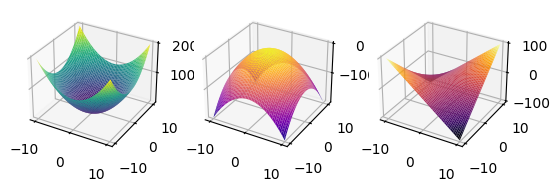
\includegraphics[width=0.5\textwidth]{pics/szelsoertek.png}
    \caption{Lokális szélsőértéktípusok}
    \label{fig:szelsoertek}
\end{figure}

\subsubsection{Hesse-mátrix}

A Hesse-mátrix a következőképpen számítható:

\begin{equation*}
    \mathbf{H(f)} = \begin{bmatrix} f''_{xx} & f''_{xy} \\ f''_{yx} & f''_{yy} \end{bmatrix} = \begin{bmatrix} \frac{\partial^2 f}{\partial x^2} & \frac{\partial^2 f}{\partial x \partial y} \\ \frac{\partial^2 f}{\partial y \partial x} & \frac{\partial^2 f}{\partial y^2} \end{bmatrix}
\end{equation*}

A Hesse mátrix determinánsa a következőket árulja el a szélsőértékről:

\begin{enumerate}
    \item Ha a determináns pozitív, akkor szélsőértéke van
    \item Ha a determináns negatív, akkor nyeregpontja van.
    \item Ha a determináns 0, akkor nem dönthető el, további vizsgálat kell.
\end{enumerate}

\vspace{4mm}

Hesse mátrix n változós függvényekre:

\begin{equation*}
    \mathbf{H(f)} = \begin{bmatrix} \frac{\partial^2 f}{\partial x_1^2} & \frac{\partial^2 f}{\partial x_1 \partial x_2} & \ldots & \frac{\partial^2 f}{\partial x_1 \partial x_n} \\ \frac{\partial^2 f}{\partial x_2 \partial x_1} & \frac{\partial^2 f}{\partial x_2^2} & \ldots & \frac{\partial^2 f}{\partial x_2 \partial x_n} \\ \vdots & \vdots & \ddots & \vdots \\ \frac{\partial^2 f}{\partial x_n \partial x_1} & \frac{\partial^2 f}{\partial x_n \partial x_2} & \ldots & \frac{\partial^2 f}{\partial x_n^2} \end{bmatrix}
\end{equation*}

\subsubsection{Lokális szélsőértékek megtalálása}

A lokális szélsőértékeket a következőképpen számíthatjuk:

\begin{enumerate}
    \item Számítsuk ki a függvény parciális deriváltjait.
    \item Rendezzük egy homogén egyenletrendszerbe a parciális deriváltakat, és oldjuk meg.
    \item Az így kapott pontok a stancionárius pontok, ahol a függvény szélsőértékei lehetnek.
    \item A stancionárius pontokat helyettesítsük a Hesse-mátrixba.
    \item Ha az első sarokfőminor ($\mathbf{H_{11}}$) és a második sarokfőminor (determináns) is pozitív, akkor \textbf{lokális minimumja van}.
    \item Ha az első sarokfőminor ($\mathbf{H_{11}}$) negatív és a második sarokfőminor (determináns) pozitív, akkor \textbf{lokális maximumja van}.
    \item Ha a determináns 0, akkor nem dönthető el, további vizsgálat kell.
\end{enumerate}

\subsubsection{Feltételes szélsőértékek megtalálása, Lagrange multiplikátor módszer}

Ha egy függvénynek egy feltétel szerint ke\-res\-sük a szél\-ső\-ér\-ték\-e\-it, ak\-kor a kö\-vet\-ke\-ző\-kép\-pen szá\-mít\-hat\-juk ki:

Legyen $f(x, y)$ a függvényünk, és legyen $g(x, y)$ a feltételünk. Ekkor a Lagrange-függvény a következőképpen néz ki:

\begin{equation*}
    L(x, y, \lambda) = f(x, y) - \lambda g(x, y)
\end{equation*}

Ezután a szélsőértékeket a következőképpen számíthatjuk:

\begin{enumerate}
    \item Számítsuk ki a Lagrange-függvény parciális deriváltjait.
    \item Rendezzük egy homogén egyenletrendszerbe a parciális deriváltakat, és oldjuk meg.
    \item Így eggyel kevesebb egyenlet van mint változó ezért a feltétel egyenletét is felhasználjuk.
    \item Megkapjuk a stancionárius pontokat, ahol az $L(x, y, \lambda)$ függvény feltétel szerinti szélsőértékei lehetnek.
    \item Behelyettesítjük a Hesse-mátrixba a stancionárius pontoka és kiértékeljük a szélsőértékeket.
\end{enumerate}

\subsection{Szintvonalak}

Egy többváltozós függvényt szintvonalakkal is le tudunk írni. A szintvonalak a következőképpen néznek ki:

\begin{equation*}
    f(x, y) = C \quad \text{ahol C egy konstans}
\end{equation*}

A szintvonalakat ábrázolva a függvény értékei egyenlőek lesznek a szintvonalakon, hiszen egy síkidom egyenletét írják le.

Ha a szintvonalak belülről kifele sűrűsödnek, és a függvény belefe növekedik, akkor a függvény konkáv, 
ha kifele növekedik, akkor konvex, ha egyenletesen sűrűsödnek, akkor egyik sem (lineáris).

\vspace{4mm}

Lehetséges hogy egy szintvonal nem létezik, vagy nincs ott megoldása a függvénynek, ekkor ott a függvény nem értelmezhető.

\subsection{Érintősík}

Míg egyváltozós függvényeknél érintőt kerestünk, kétváltozósnál érintősíkot kerestünk. Az érintősík egy adott pontban érinti a függvényt, és a függvény értékének a változását mutatja az adott pontban.

\vspace{4mm}

Az érintősík egyenlete a következőképpen számítható $P(x_0,y_0,z_0)$ pontban:

\begin{equation*}
    z = f(x_0, y_0) + f'_x(x_0, y_0)(x - x_0) + f'_y(x_0, y_0)(y - y_0)
\end{equation*} 

Ezt nullára rendezve megkapjuk az é\-rin\-tő\-sík e\-gyen\-let\-ét. Az é\-rin\-tő\-sík nor\-mál\-vek\-to\-ra a kö\-vet\-ke\-ző\-kép\-pen számítható:

\begin{equation*}
    \mathbf{n} = \begin{bmatrix} f'_x(x_0, y_0) \\ f'_y(x_0, y_0) \\ -1 \end{bmatrix}
\end{equation*}

\newpage

\subsection{Gradiens}

A gradiens egy olyan vektor, ami a függvény értékének a változását mutatja az adott pontban. A gradiens a következőképpen számítható:

\begin{equation*}
    \underline{\nabla} f = \begin{bmatrix} \frac{\partial f}{\partial x_1} \\ \frac{\partial f}{\partial x_2} \\ \vdots \\ \frac{\partial f}{\partial x_n} \end{bmatrix}
\end{equation*}

A gradiens iránya a legnagyobb növekedés iránya, a gradiens hossza pedig a legnagyobb növekedés mértéke.

\vspace{4mm}

Az iránymenti deriváltakat a gradiens segítségével számíthatjuk:

\begin{equation*}
    \frac{\partial f}{\partial \mathbf{v}} = \underline{\nabla} f \cdot \underline{v}
\end{equation*}

Ahol $\underline{v}$ a vizsgált irány vektora. Ha $\underline{v}$ nem egységnyi hosszú, akkor el kell osztani a saját hosszával:

\begin{equation*}
    \frac{\partial f}{\partial \mathbf{v}} = \frac{\underline{\nabla} f \cdot \underline{v}}{\left\lVert \underline{v} \right\rVert}
\end{equation*}

\subsection{Implicit függvények deriválása}

Egy $F(x,y)=0$ implicit függvény deriválását a következőképpen számíthatjuk:

\begin{equation*}
    y' = \frac{\partial y}{\partial x} = -\frac{\frac{\partial F}{\partial x}}{\frac{\partial F}{\partial y}}
\end{equation*}

\begin{equation*}
    x' = \frac{\partial x}{\partial y} = -\frac{\frac{\partial F}{\partial y}}{\frac{\partial F}{\partial x}}
\end{equation*}

Fontos hogy $F(x,y) = 0$ nem kétváltozós függvény, hanem egyenlet, ezért a deriválásnál figyelni kell a változókra.
 Tehát ezzel a módszerrel a Matematika 1.-ben tanult implicit deriválást tudjuk alkalmazni egyszerűbben. 

\vspace{4mm}

Ez akár n változós implicit függvényekre is alkalmazható:

\begin{equation*}
    x_i' = \frac{\partial x_i}{\partial x_j} = -\frac{\frac{\partial F}{\partial x_j}}{\frac{\partial F}{\partial x_i}}
\end{equation*}

\newpage

\subsection{Többváltozós függvények határértékszámítása}

\subsubsection{Definció kétváltozós függvényekre}

B az $f(x,y)$ határértéke a $(x_0, y_0)$ pontban, ha minden $\varepsilon  > 0$-hoz létezik $\delta > 0$ úgy, hogy ha $(x,y) \in B_{\delta}((x_0, y_0))$ és $(x,y) \neq (x_0, y_0)$, vagyis:

\begin{equation*}
    0 < \sqrt{(x-x_0)^2 + (y-y_0)^2} < \delta
\end{equation*}

ekkor:

\begin{equation*}
    \left\lvert f(x,y) - B \right\rvert < \varepsilon
\end{equation*}

\vspace{4mm}

Ezeknél a feladatoknál hasznos lehet a háromszög egyenlőtlenség:

\begin{equation*}
    \left\lvert a + b \right\rvert \leq \left\lvert a \right\rvert + \left\lvert b \right\rvert
\end{equation*}

\subsubsection{Egyszerűbb határértékek számítása}

Lehetséges (nem ezen az egyetemen), hogy behelyettesítjük x-et és y-t és létezik a határérték:

\begin{equation*}
    \lim_{(x,y) \to (x_0, y_0)} f(x,y) = f(x_0, y_0)  =B
\end{equation*}

\vspace{4mm}

Ha polinom/polinom függvényünk van ak\-kor né\-ha a \textbf{szor\-zattá a\-lak\-ít\-ás} se\-gít\-het:

\begin{equation*}
    \lim_{(x,y) \to (4, 0)} \frac{x^2 y -4xy}{yx^2 -16y} = \lim_{(x,y) \to (4, 0)} \frac{y(x^2-4x)}{y(x^2 -16)} = \lim_{(x,y) \to (4, 0)} \frac{x}{x-4} = \frac{1}{2}
\end{equation*}

\subsubsection{Egyenes mentén való határérték számítása}

Veszünk egy $y = mx + b$ egyenest ami érinti $x$-et és $y$-t, és ezen az egyenesen szá\-mol\-juk a határ\-ér\-téket. Ek\-kor a kö\-vet\-ke\-ző\-kép\-pen számíthatjuk a határértéket:

\begin{equation*}
    \lim_{(x,y) \to (x_0, y_0)} f(x,y) = \lim_{x \to x_0} f(x, mx + b)
\end{equation*}

Itt sajnos ahhoz hogy létezzen a határérték, minden $m$ értékre a ha\-tár\-ér\-ték\-nek ugyanaznak kell lennie. Ha ez nem teljesül, akkor a határérték nem létezik. 
De ha nem függ $m$-től, akkor a határérték létezik. Ne felejtsük el a konstans egyenest se.

%TODO lecsekkolni hogy jó-e

\subsubsection{Átviteli elv}

Ha egy függvény egyenletesen konvergens egy sorozatban, akkor a határértéke a függvénynek a sorozat határértékével egyenlő.

\vspace{4mm}

Ennek gyakori fajtáka a polárkoordinátás helyettesítés:

\begin{equation*}
    x = \rho \cos(\phi) \quad y = \rho \sin(\phi) \quad \rho \to 0 \quad \phi = \text{tetszőleges konstans}
\end{equation*}

Ezeket felhasználva a határértéket könnyen ki tudjuk számolni (mivel a $\cos(\phi)$, és a $\sin(\phi)$ véges).

\subsection{Totális és parciális deriválhatóság}

Az $f(x,y)$ függvény totálisan deriválható $(x_0, y_0)$ helyen ha $\exists A,B \in \mathbb{R}$ amire igaz, hogy:

\begin{equation*}
    \lim_{(x,y) \to (x_0, y_0)} \frac{f(x,y) - (A(x-x_0) + B(y-y_0) + f(x_0, y_0))}{\sqrt{(x-x_0)^2 + (y-y_0)^2}} = 0
\end{equation*}

Ha itt a határértkben $y$-t $y_0$-nak vagy $x$-et $x_0$-nak vá\-laszt\-juk, ak\-kor a par\-ci\-á\-lis de\-ri\-vál\-ta\-kat kapjuk:

\begin{equation*}
    \lim_{x \to x_0} \frac{f(x,y_0) - f(x_0, y_0)}{x-x_0} = A
\end{equation*}

\begin{equation*}
    \lim_{y \to y_0} \frac{f(x_0,y) - f(x_0, y_0)}{y-y_0} = B
\end{equation*}

Itt az A és B értékek a függvény parciális deriváltjai a $(x_0, y_0)$ pontban, amiket az érintősík egyenletében is használhatunk.

\begin{equation*}
    f(x,y) \text{ totálisan deriválható } \Rightarrow f(x,y) \text{ parciálisan is deriválható}
\end{equation*}

Ez fordítva nem igaz, tehát ha a függvény parciálisan deriválható, akkor nem biztos hogy totálisan is deriválható.

\subsubsection{Young tétel}


\begin{equation*}
    f(x,y) \text{ kétszer totálisan deriválható } \Leftrightarrow \frac{\partial^2 f}{\partial x \partial y} = \frac{\partial^2 f}{\partial y \partial x}
\end{equation*}


\newpage

\section{Többváltozós függvények integrálása}

\subsection{Kettős integrál}

Mígy az egyváltozós integrál a függvény alatti területet számolta, addig a kettős integrál a függvény alatti test térfogatot számolja.

\begin{equation*}
    \int_{a}^{b} \int_{c}^{d} f(x,y) dy dx = \int_{c}^{d} \int_{a}^{b} f(x,y) dx dy
\end{equation*}

Az integrálás sorrendje tetszőleges, viszont figyelni kell hogy a határok is megfelelőek legyenek.

\subsubsection{Kettős integrál számítása téglalap alakú tartományon}

A kettős integrált elkezdjük a belső integrálással, majd a kül\-ső in\-teg\-rá\-lás\-sal számoljuk ki.
Ilyenkor a külső integrálás változója konstansnak számít, és ugyanúgy integráljuk. Amint megvan a primitív függvény, behelyettesítjük az első integrálás határait
és integrálunk a külső változó szerint.

Példa egy ilyen integrálra:

\begin{equation*}
    \int_{0}^{1} \int_{0}^{2} (x^2 + y) dy dx = \int_{0}^{1} \left[ x^2y + \frac{y^2}{2} \right]_{0}^{2} dx = \int_{0}^{1} (2x^2 + 2) dx = \left[ \frac{2x^3}{3} + 2x \right]_{0}^{1} = \frac{8}{3}
\end{equation*}

\subsubsection{Kettős integrál számítása normáltartományon}

Ha a tartomány nem téglalap alakú, akkor a következőképpen számíthatjuk a kettős integrált:

\begin{equation*}
    \iint_{D} f(x,y) dx dy = \int_{a}^{b} \int_{g(x)}^{h(x)} f(x,y) dy dx
\end{equation*}

Ahol $g(x)$ és $h(x)$ a tartomány $x$ tengely menti határai és $D$ a tartomány. Ilyenkor a belső integrálásban a $y$-tól (amelyik nem tartalmaz változót) függő határokat kell behelyettesíteni.

A tengely menti határokat úgy kapjuk meg, hogy a tartományt a $y = g(x)$ és $y = h(x)$ függvényekkel határoljuk.

\subsubsection{Kettős integrál határai}

Sokszor érdemes az integrálás megkezdése előtt megnézni, hogy esetleg a a határok cseréjével egyszerűsíthető-e az integrál.

Például:

\begin{equation*}
    \int_{0}^{1} \int_{1}^{2} \frac{2x\arcsin(xy)}{\sqrt{1+ {(xy)}^2}} dx dy =\int_{1}^{2} \int_{0}^{1} \frac{2x\arcsin(xy)}{\sqrt{1+ {(xy)}^2}} dy dx 
\end{equation*}

Itt jóval egyszerűbb először a $y$ szerint integrálni, hiába eredetileg $x$ szerint volt megadva.

\subsubsection{Helyettesítéses integrálás}

Helyettesítéses integrálásnál ha egy $x=x(u,v)$ és $y=y(u,v)$ 
helyettesítést végzünk, akkor a Jacobi-féle determináns abszolút értékének segítségével tudjuk a kettős integrált átalakítani
 (fontos, hogy a determináns nem lehet nulla).

\begin{equation*}
    \iint_{D} f(x,y) dx dy = \iint_{D_{uv}} f(x(u,v), y(u,v)) \left| \frac{\partial(x,y)}{\partial(u,v)} \right| du dv
\end{equation*}

Ahol a Jacobi-féle determináns a következőképpen számítható:

\begin{equation*}
    \left| \frac{\partial(x,y)}{\partial(u,v)} \right| = \left| \begin{bmatrix} \frac{\partial x}{\partial u} & \frac{\partial x}{\partial v} \\ \frac{\partial y}{\partial u} & \frac{\partial y}{\partial v} \end{bmatrix} \right| = \left| \frac{\partial x}{\partial u} \frac{\partial y}{\partial v} - \frac{\partial x}{\partial v} \frac{\partial y}{\partial u} \right|
\end{equation*}

\subsubsection{Kettős integrál számítása polárkoordinátákban}

Ha mondjuk egy kör alakú tartományban szeretnénk számolni a kettős integrált (de sok más esetben is), akkor érdemes polárkoordinátákat használni.

\begin{equation*}
    x = r \cos(\phi) \quad y = r \sin(\phi) \quad r \in [0, R] \quad \phi \in [0, 2\pi]
\end{equation*}

Ahol $r$ a sugarat, $\phi$ pedig a szöget, az R pedig a kör sugarát jelöli. Ekkor a kettős integrált a következőképpen számítható:

\begin{equation*}
    \iint_{D} f(x,y) dx dy = \int_{0}^{2\pi} \int_{0}^{R} r f(r \cos(\phi), r \sin(\phi)) dr d\phi
\end{equation*}

Itt azért szorozzuk $r$-rel a függvényt, mert a Jacobi-féle determináns abszolút értéke ilyenkor $r$.

\newpage

\subsection{Hármas integrál}

A hármas integrál már inkabb fizikai alkalmazásokban fordul elő, ezzel például 
térfogatot, nyomást, sűrűséget, vagy töltéseloszlást lehet számolni.

\subsubsection{Hármas integrál számítása téglalap alakú tartományon}

A hármas integrálás ugyanúgy működik mint a kettős, téglalap alapú tar\-to\-mány\-on, csak itt már 3 dimenzióban számolunk.

\begin{equation*}
    \iiint_{D} f(x,y,z) dx dy dz = \int_{a}^{b} \int_{c}^{d} \int_{e}^{g} f(x,y,z) dz dy dx
\end{equation*}

\subsubsection{Hármas integrál számítása normáltartományon}

Ha a tartomány nem téglalap alakú, akkor a következőképpen számíthatjuk a hármas integrált:

\begin{equation*}
    \iiint_{D} f(x,y,z) dx dy dz = \int_{a}^{b} \int_{g(x)}^{h(x)} \int_{p(x,y)}^{q(x,y)} f(x,y,z) dz dy dx
\end{equation*}

Ahol $g(x)$ és $h(x)$ a tartomány $x$ tengely menti határai, $p(x,y)$ és $q(x,y)$ a tartomány $y$ tengely menti határai és $D$ a tartomány.

\subsubsection{Helyettesítéses integrálás}

Helyettesítéses integrálásnál ha egy $x=x(u,v,w)$, $y=y(u,v,w)$ és $z=z(u,v,w)$

helyettesítést végzünk, akkor a Jacobi-féle determináns abszolút értékének segítségével tudjuk a hármas integrált átalakítani
 (fontos, hogy a determináns nem lehet nulla).

\begin{equation*}
    \iiint_{D} f(x,y,z) dx dy dz =
\end{equation*}


\begin{equation*}
    \iiint_{D_{uvw}} f(x(u,v,w), y(u,v,w), z(u,v,w)) \left| \frac{\partial(x,y,z)}{\partial(u,v,w)} \right| du dv dw
\end{equation*}

Ahol a Jacobi-féle determináns a következőképpen számítható:

\begin{equation*}
    \left| \frac{\partial(x,y,z)}{\partial(u,v,w)} \right| = \left| \begin{bmatrix} \frac{\partial x}{\partial u} & \frac{\partial x}{\partial v} & \frac{\partial x}{\partial w} \\ \frac{\partial y}{\partial u} & \frac{\partial y}{\partial v} & \frac{\partial y}{\partial w} \\ \frac{\partial z}{\partial u} & \frac{\partial z}{\partial v} & \frac{\partial z}{\partial w} \end{bmatrix} \right|
\end{equation*}

\newpage

\subsubsection{Hármas integrál számítása hengerkoordinátákban}

Ha henger alakú tartományban szeretnénk számolni a hármas integrált, akkor érdemes hengerkoordinátákat használni.

\begin{equation*}
    x = r \cos(\phi) \quad y = r \sin(\phi) \quad z = z \quad r \in [0, R] \quad \phi \in [0, 2\pi] \quad z \in [a, b]
\end{equation*}

Szerencsére a Jacobi-féle determináns itt is $r$, így a hármas integrált a következőképpen számítható:

\begin{equation*}
    \iiint_{D} f(x,y,z) dx dy dz = \int_{a}^{b} \int_{0}^{2\pi} \int_{0}^{R} r f(r \cos(\phi), r \sin(\phi), z) dr d\phi dz
\end{equation*}

\subsubsection{Hármas integrál számítása gömbkoordinátákban}

Ha gömb alakú tartományban szeretnénk számolni a hármas integrált, akkor érdemes gömbkoordinátákat használni.

\begin{equation*}
    x = r \sin(\theta) \cos(\phi) \quad y = r \sin(\theta) \sin(\phi) \quad z = r \cos(\theta)
\end{equation*}

\begin{equation*}
    r \in [0, R] \quad \phi \in [0, 2\pi] \quad \theta \in [0, \pi]
\end{equation*}

A Jacobi-féle determináns itt $r^2 \sin(\theta)$, így a hármas integrált a kö\-vet\-ke\-ző\-kép\-pen számítható:

\begin{equation*}
    \iiint_{D} f(x,y,z) dx dy dz =
\end{equation*}

\begin{equation*}
    \int_{0}^{2\pi} \int_{0}^{\pi} \int_{0}^{R} r^2 \sin(\theta) f(r \sin(\theta) \cos(\phi), r \sin(\theta) \sin(\phi), r \cos(\theta)) dr d\theta d\phi
\end{equation*}

\end{document}